\documentclass[../physics12.tex]{subfiles}
\graphicspath{{\subfix{../figures/}}}
\begin{document}

\chapter{Electromagnetic Waves and Wave Optics}
\section{Formulas for Chapter 13 and Chapter 14}
Note these are for this chapter and the next chapter.

EM waves in vacuum: $E/B = c = 1/\sqrt{\mu_0 \epsilon_0}$

Relationship between wavelength and frequency: $c=\lambda f$

Intensity of EM wave: $I = \text{Power}/\text{Area} = \frac{E_{\text{max}}B_\text{max}}{2\mu_0}$

Intensity of point source at distance, $r$: $I = \frac{\text{Power}}{4\pi r^2}$

Power: $P = \Delta E/\Delta t$

Index of refraction: $n=c/v=\lambda_0/\lambda_n$

Regular reflection: $\theta_{\text{incident}}=\theta_{\text{reflected}}$

Snell's law of refraction: $n_1\sin\theta_1 = n_2\sin\theta_2$

Critical angle for total internal reflection: $\sin\theta_c = n_2/n_1$

Ray tracing rules:

Mirror: Ray arriving at center of sphere (axis) reflects symmetrically. Ray parallel to axis, converges towards F (or diverges away from F), $f=R/2$

Lens: Ray through center of lens, undeflected. Ray parallel to axis, converges toward F (or diverges away from F).

Image: $d_i>0$ (real), $d_i<0$ (virtual)

Focal point $f$: at $d_0=\infty$, $d_i=f$ 
\begin{center}
    $f = \pm |f|$, ``+'' convergent, ``-'' divergent 
\end{center}

Magnification: $M=h_i/h_0 = -d_i/d_0$

Power of a lens: $P=1/f$

Two-lens magnification: $M=M_1M_2$

Telescope angular magnification: $M=\theta'/\theta = -f_0/f_e$

Double slit interference: $d\sin\theta_{\text{bright}} = m\lambda$, $d\sin\theta_{\text{dark}} = (m+1/2)\lambda$

Single slit diffraction minima: $a\sin\theta_{\text{dark}} = m\lambda$

Small angle approximation: $\sin\theta \approx \tan\theta = y/L$

Grating maxima: $d\sin\theta_{\text{bright}} = m\lambda$

Reflection phase change: 180$\degree$ from denser medium (larger $n$) and $0\degree$ from lighter medium (smaller $n$)

Malaus' law for polarized EM wave or light: $I=I_0\cos^2\theta$

Polarization by reflection: Brewster's angle: $\tan\theta_b = n_2/n_1$

Unpolarized EM wave or light through a polarizer: $I=I_0/2$

Rayleigh's criterion for a circular aperture: $\theta_{\text{min}} = 1.22\lambda/D$

\section{Power from a Radio Transmitter Problem}
The amplitude of the electric field is 0.7 V/m 10 km from a radio transmitter.

What is the total power emitted by the transmitter, if one assumes that the radiation is emitted isotropically (uniformly in all directions)? The 
impedence of free space is 377 $\Omega$. Answer in units of W.

\section{Energy from the Sun through a Window Problem}
The average energy per unit time per unit area that reaches the upper atmosphere of the Earth from the Sun, called the solar constant, is 1.35 kW/m$^2$.
Because of absorption and reflection by the atmosphere, about 0.2 kW/m$^2$ reaches the surface of the earth on a clear day.

How much energy is collected during 2 h of daylight by a window that measures 1.2 m by 1.4 m? The window is on a mount that rotates, keeping the window facing the sun 
so the sun's rays remain perpendicular to the window. Answer in units of MJ.

\section{High Power Laser Problem}
High power lasers in factories are used to cut through cloth and metal. One such laser has a beam diameter of 0.825 mm and generates an electric field at the target having an amplitude of 1.02 MV/m.
The speed of light is $2.99792\times 10^8$ m/s the permeability of free space is $4\pi \times 10^{-7}$ T$\cdot$N/A.

(a) What is the amplitude of the magnetic field produced? Answer in units of T.

(b) What is the intensity of the laser? Answer in units of W/m$^2$.

(c) What is the power dissipated? Answer in units of W.

\section{EMF in Receiving Antenna Problem}
An AM radio station broadcasts with an average power of 3.6 kW. A dipole receiving antenna 62.5 cm long is located 1.7 km from the transmitter. 
Assume the transmitter is a point source, the waves are traveling perpendicular to the axis of the receiving antenna, and that the source is far enough away that the wave 
amplitude is constant along the receiving antenna.

Compute the amplitude of the induced emf by this signal between the ends of the receiving antenna. $\mu_0 c = 377 \Omega$ and 1.609 km = 1 mi. Answer in units of V.

\section{Microwave Transmitter Problem}
A microwave transmitter emits electromagnetic waves of a single wavelength. The maximum electric field 1.44 km from the transmitter is 8.39 V/m. The speed of light 
is $2.99792\times 10^8$ m/s and the permeability of free space is $4\pi \times 10^{-7}$ N/A$^2$. 

(a) Assuming that the transmitter is a point source and neglecting waves reflected from the Earth, calculate the maximum magnetic field at this distance. Answer in units of T.

(b) Calculate the total power emitted by the transmitter. Answer in units of W.

\section{Three Polarizers Problem}
Three polarizing disks whose planes are parallel are centered on a common axis. The directions of the transmission axes relative to the common vertical direction are shown.
A linearly polarized beam of light with the plane of polarization parallel to the vertical reference direction is incident from the left on the first disk with intensity $I_i = 7.62$ units (arbitrary).
\begin{center}
    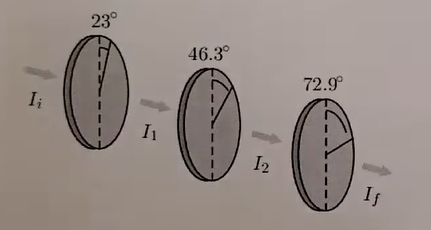
\includegraphics[width=0.5\textwidth]{13.1.PNG}
\end{center}
Calculate the transmitted intensity $I_f$ when $\theta_1 = 23\degree$, $\theta_2 = 46.3\degree$, and $\theta_3 = 72.9\degree$.

\section{Two Glass Plates Problem}
A hair is placed at one edge between two flat glass plates 10.3 cm long. When this arrangement is illuminated with 541 nm light, 120 bands are counted, starting at the point of contact of the two plates.

How thick is the hair? Answer in units of m.

\section{Satellite Problem}
A converging lens with a diameter of 41.5 cm forms an image of a satellite passing overhead. The satellite has two green lights (wavelength 492 nm) spaces 0.9 m apart. 

If the lights can just be resolved according to the Rayleigh criterion, what is the altitude of the satellite? Answer in units of km.


\end{document}